\documentclass[12pt,a4paper]{report}

% ============================================================================
% PACKAGES
% ============================================================================
\usepackage[utf8]{inputenc}
\usepackage[T1]{fontenc}
\usepackage{lmodern}
\usepackage[margin=1in]{geometry}
\usepackage{graphicx}
\usepackage{xcolor}
\usepackage{hyperref}
\usepackage{tikz}
\usepackage{longtable}
\usepackage{booktabs}
\usepackage{fancyhdr}
\usepackage{titlesec}
\usepackage{listings}
\usepackage{enumitem}

% TikZ Libraries
\usetikzlibrary{shapes.geometric, arrows.meta, positioning, fit, backgrounds, 
                decorations.pathreplacing, calc}

% ============================================================================
% COLORS
% ============================================================================
\definecolor{primaryblue}{RGB}{26, 54, 93}
\definecolor{secondaryblue}{RGB}{59, 130, 246}
\definecolor{accentgreen}{RGB}{34, 197, 94}
\definecolor{warningorange}{RGB}{249, 115, 22}
\definecolor{lightgray}{RGB}{243, 244, 246}
\definecolor{darkgray}{RGB}{75, 85, 99}
\definecolor{codebg}{RGB}{249, 250, 251}

% ============================================================================
% HYPERREF SETUP
% ============================================================================
\hypersetup{
    colorlinks=true,
    linkcolor=primaryblue,
    urlcolor=secondaryblue,
    pdftitle={EduX - System Architecture},
    pdfauthor={EduX Development Team},
}

% ============================================================================
% HEADER/FOOTER
% ============================================================================
\pagestyle{fancy}
\fancyhf{}
\fancyhead[L]{\textcolor{darkgray}{\small EduX School Management System}}
\fancyhead[R]{\textcolor{darkgray}{\small Architecture Documentation}}
\fancyfoot[C]{\textcolor{darkgray}{\thepage}}
\renewcommand{\headrulewidth}{0.4pt}

% ============================================================================
% TITLE FORMATTING
% ============================================================================
\titleformat{\chapter}[display]
  {\normalfont\huge\bfseries\color{primaryblue}}
  {\chaptertitlename\ \thechapter}{20pt}{\Huge}

\titleformat{\section}
  {\normalfont\Large\bfseries\color{primaryblue}}
  {\thesection}{1em}{}

\titleformat{\subsection}
  {\normalfont\large\bfseries\color{secondaryblue}}
  {\thesubsection}{1em}{}

% ============================================================================
% LISTINGS SETUP
% ============================================================================
\lstset{
    backgroundcolor=\color{codebg},
    basicstyle=\ttfamily\small,
    breaklines=true,
    frame=single,
    rulecolor=\color{darkgray!30},
    language=bash,
}

% ============================================================================
% DOCUMENT
% ============================================================================
\begin{document}

% ----------------------------------------------------------------------------
% TITLE PAGE
% ----------------------------------------------------------------------------
\begin{titlepage}
    \centering
    \vspace*{2cm}
    
    {\Huge\bfseries\textcolor{primaryblue}{EduX}\par}
    \vspace{0.5cm}
    {\Large\textcolor{secondaryblue}{School Management System}\par}
    
    \vspace{2cm}
    
    
\begin{tikzpicture}
        \node[draw=primaryblue, line width=2pt, rounded corners=10pt, 
              minimum width=8cm, minimum height=3cm, fill=lightgray] 
              {\Huge\bfseries\textcolor{primaryblue}{System Architecture}};
    \end{tikzpicture}
    
    \vspace{1cm}
    {\large\textcolor{darkgray}{\textit{Developer Documentation}}\par}
    
    \vfill
    
    {\large\textcolor{darkgray}{Version 1.0}\par}
    {\large\textcolor{darkgray}{\today}\par}
\end{titlepage}

\tableofcontents
\newpage

% ============================================================================
% CHAPTER 1: OVERVIEW
% ============================================================================
\chapter{Architecture Overview}

\section{Introduction}

EduX is built using a clean, layered architecture that separates concerns and promotes maintainability. The application follows the Presentation-Domain-Data pattern with Riverpod for state management.

\section{Technology Stack}

\begin{longtable}{@{}p{4cm}p{9cm}@{}}
\toprule
\textbf{Component} & \textbf{Technology} \\
\midrule
\endhead
Framework & Flutter 3.x (Desktop - Windows) \\
Language & Dart 3.x \\
Database & SQLite via Drift ORM \\
State Management & Riverpod 2.x \\
Navigation & go\_router \\
PDF Generation & pdf + printing packages \\
Excel Support & excel package \\
Charts & fl\_chart \\
\bottomrule
\end{longtable}

\section{Three-Layer Architecture}

\begin{center}
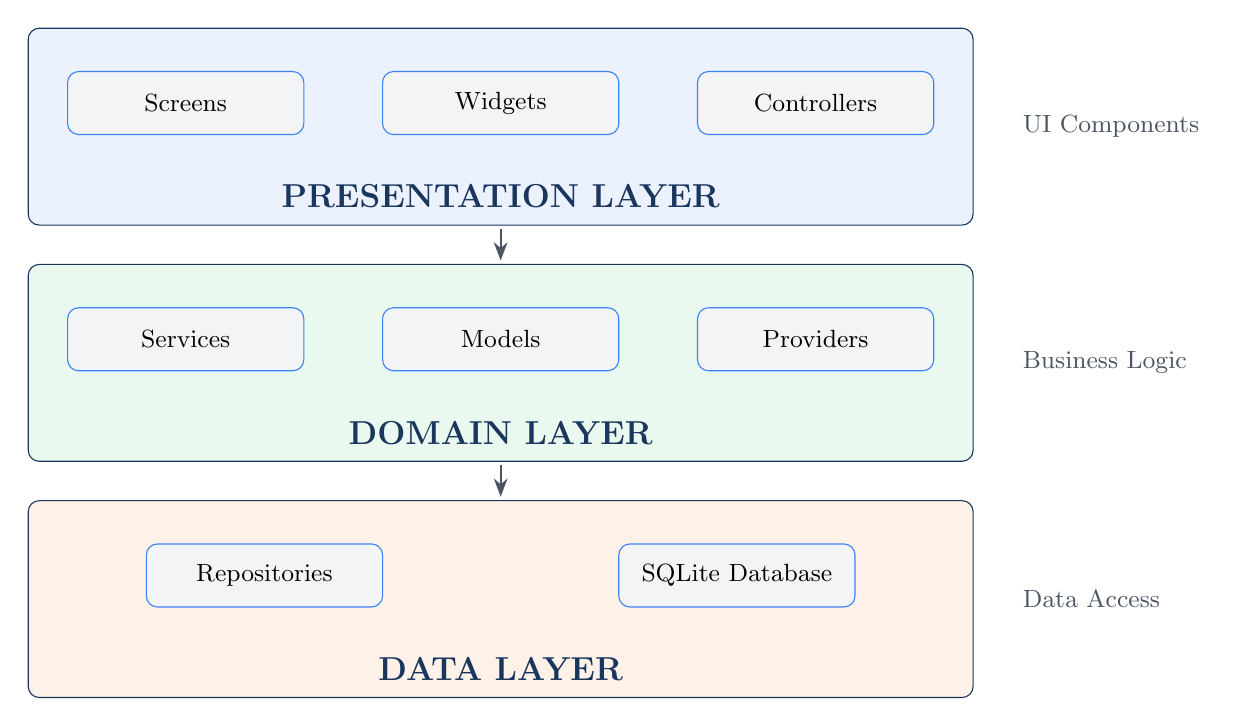
\begin{tikzpicture}[
    layer/.style={draw=primaryblue, rounded corners, minimum width=12cm, 
                  minimum height=2.5cm, align=center},
    component/.style={draw=secondaryblue, rounded corners, minimum width=3cm, 
                      minimum height=0.8cm, fill=lightgray, font=\small},
    arrow/.style={-{Stealth}, thick, darkgray}
]
    % Presentation Layer
    \node[layer, fill=secondaryblue!10] (presentation) at (0,6) {};
    \node[above=0.1cm of presentation.south, font=\bfseries\large, 
          text=primaryblue] {PRESENTATION LAYER};
    \node[component] at (-4,6.3) {Screens};
    \node[component] at (0,6.3) {Widgets};
    \node[component] at (4,6.3) {Controllers};
    
    % Domain Layer
    \node[layer, fill=accentgreen!10] (domain) at (0,3) {};
    \node[above=0.1cm of domain.south, font=\bfseries\large, 
          text=primaryblue] {DOMAIN LAYER};
    \node[component] at (-4,3.3) {Services};
    \node[component] at (0,3.3) {Models};
    \node[component] at (4,3.3) {Providers};
    
    % Data Layer
    \node[layer, fill=warningorange!10] (data) at (0,0) {};
    \node[above=0.1cm of data.south, font=\bfseries\large, 
          text=primaryblue] {DATA LAYER};
    \node[component] at (-3,0.3) {Repositories};
    \node[component] at (3,0.3) {SQLite Database};
    
    % Arrows
    \draw[arrow] (0,4.7) -- (0,4.3);
    \draw[arrow] (0,1.7) -- (0,1.3);
    
    % Labels
    \node[right=0.5cm of presentation.east, font=\small, text=darkgray] 
        {UI Components};
    \node[right=0.5cm of domain.east, font=\small, text=darkgray] 
        {Business Logic};
    \node[right=0.5cm of data.east, font=\small, text=darkgray] 
        {Data Access};
\end{tikzpicture}
\end{center}

% ============================================================================
% CHAPTER 2: PRESENTATION LAYER
% ============================================================================
\chapter{Presentation Layer}

\section{Overview}

The Presentation Layer handles all UI-related code including screens, widgets, and user interaction logic.

\section{Directory Structure}

\begin{lstlisting}
lib/
|-- screens/           # Full-page screens
|   |-- students/      # Student module screens
|   |-- attendance/    # Attendance screens
|   |-- fees/          # Fee management screens
|   |-- exams/         # Examination screens
|   |-- staff/         # Staff management screens
|   |-- academics/     # Academic screens
|   |-- guardians/     # Guardian screens
|
|-- features/          # Feature-specific widgets
|   |-- dashboard/     # Dashboard components
|   |-- settings/      # Settings screens
|   |-- auth/          # Authentication UI
|   |-- shell/         # App shell with navigation
|
|-- core/
    |-- widgets/       # Shared/reusable widgets
    |-- theme/         # Theme configuration
\end{lstlisting}

\section{Screen Architecture}

\begin{center}
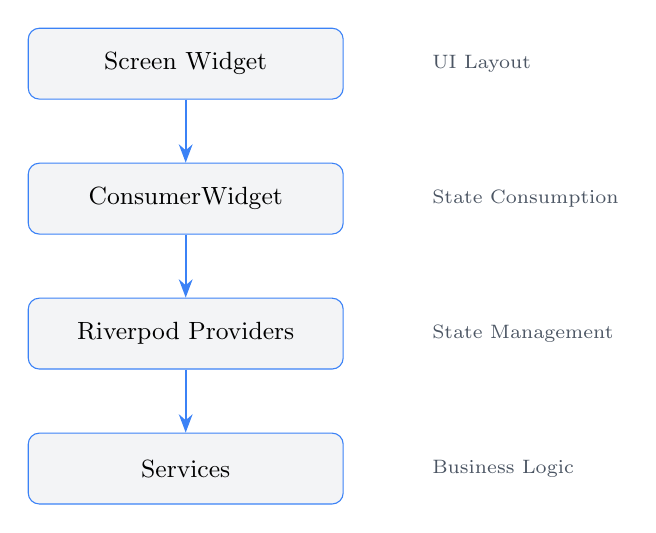
\begin{tikzpicture}[
    node distance=0.8cm,
    box/.style={draw=secondaryblue, rounded corners, minimum width=4cm, 
                minimum height=0.9cm, fill=lightgray, font=\small},
    arrow/.style={-{Stealth}, thick, secondaryblue}
]
    \node[box] (screen) {Screen Widget};
    \node[box, below=of screen] (consumer) {ConsumerWidget};
    \node[box, below=of consumer] (provider) {Riverpod Providers};
    \node[box, below=of provider] (service) {Services};
    
    \draw[arrow] (screen) -- (consumer);
    \draw[arrow] (consumer) -- (provider);
    \draw[arrow] (provider) -- (service);
    
    \node[right=1cm of screen, font=\scriptsize, text=darkgray] 
        {UI Layout};
    \node[right=1cm of consumer, font=\scriptsize, text=darkgray] 
        {State Consumption};
    \node[right=1cm of provider, font=\scriptsize, text=darkgray] 
        {State Management};
    \node[right=1cm of service, font=\scriptsize, text=darkgray] 
        {Business Logic};
\end{tikzpicture}
\end{center}

\section{Navigation with go\_router}

The application uses \texttt{go\_router} for declarative routing with nested navigation.

\subsection{Route Structure}

\begin{lstlisting}
/                     # Splash screen
/login                # Authentication
/setup                # First-time setup
/app                  # Main app shell
  /app/dashboard      # Dashboard
  /app/students       # Student listing
  /app/students/:id   # Student details
  /app/attendance     # Attendance
  /app/fees           # Fee management
  /app/exams          # Examinations
  /app/staff          # Staff management
  /app/settings       # Settings
\end{lstlisting}

% ============================================================================
% CHAPTER 3: DOMAIN LAYER
% ============================================================================
\chapter{Domain Layer}

\section{Services}

Services contain business logic and orchestrate data operations.

\begin{center}
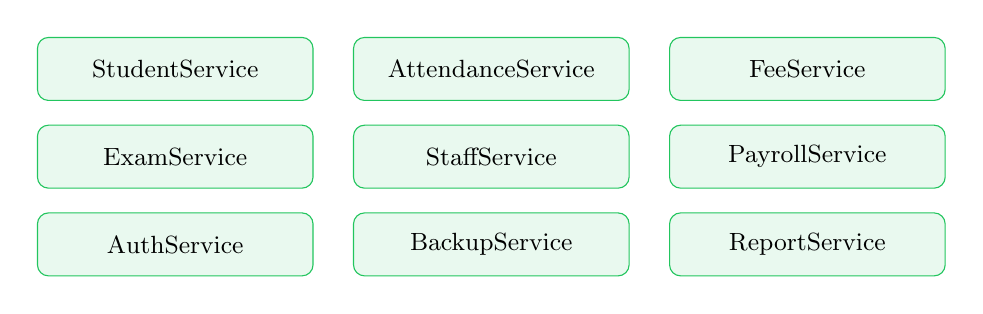
\begin{tikzpicture}[
    service/.style={draw=accentgreen, rounded corners, minimum width=3.5cm, 
                    minimum height=0.8cm, fill=accentgreen!10, font=\small}
]
    \matrix[row sep=0.3cm, column sep=0.5cm] {
        \node[service] {StudentService}; & 
        \node[service] {AttendanceService}; & 
        \node[service] {FeeService}; \\
        \node[service] {ExamService}; & 
        \node[service] {StaffService}; & 
        \node[service] {PayrollService}; \\
        \node[service] {AuthService}; & 
        \node[service] {BackupService}; & 
        \node[service] {ReportService}; \\
    };
\end{tikzpicture}
\end{center}

\subsection{Service Responsibilities}

\begin{longtable}{@{}p{4cm}p{9cm}@{}}
\toprule
\textbf{Service} & \textbf{Responsibilities} \\
\midrule
\endhead
StudentService & CRUD operations, enrollment, status management \\
AttendanceService & Mark attendance, alerts, statistics \\
FeeService & Fee structure, concessions \\
InvoiceService & Generate, update invoices \\
PaymentService & Record payments, receipts \\
ExamService & Exam CRUD, marks, results \\
StaffService & Staff CRUD, assignments \\
PayrollService & Salary calculation, processing \\
AuthService & Login, logout, password management \\
BackupService & Create, restore backups \\
ReportService & Generate various reports \\
\bottomrule
\end{longtable}

\section{Providers (Riverpod)}

Providers manage application state and expose data to the UI.

\subsection{Provider Types Used}

\begin{longtable}{@{}p{4cm}p{9cm}@{}}
\toprule
\textbf{Provider Type} & \textbf{Use Case} \\
\midrule
\endhead
Provider & Simple computed values, services \\
StateProvider & Simple mutable state \\
FutureProvider & Async data fetching \\
StreamProvider & Real-time data streams \\
StateNotifierProvider & Complex state with mutations \\
\bottomrule
\end{longtable}

\subsection{Provider Architecture}

\begin{center}
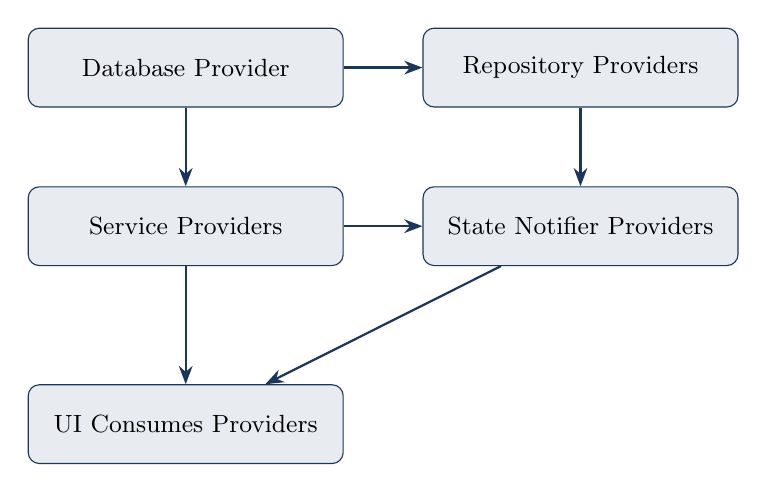
\begin{tikzpicture}[
    node distance=1cm,
    prov/.style={draw=primaryblue, rounded corners, minimum width=4cm, 
                 minimum height=1cm, fill=primaryblue!10, align=center, 
                 font=\small},
    arrow/.style={-{Stealth}, thick, primaryblue}
]
    \node[prov] (db) {Database Provider};
    \node[prov, right=1cm of db] (repo) {Repository Providers};
    \node[prov, below=of db] (service) {Service Providers};
    \node[prov, below=of repo] (state) {State Notifier Providers};
    \node[prov, below=1.5cm of service] (ui) {UI Consumes Providers};
    
    \draw[arrow] (db) -- (repo);
    \draw[arrow] (repo) -- (state);
    \draw[arrow] (db) -- (service);
    \draw[arrow] (service) -- (state);
    \draw[arrow] (state) -- (ui);
    \draw[arrow] (service) -- (ui);
\end{tikzpicture}
\end{center}

% ============================================================================
% CHAPTER 4: DATA LAYER
% ============================================================================
\chapter{Data Layer}

\section{Drift ORM}

Drift provides type-safe database access with code generation.

\subsection{Key Features}

\begin{itemize}[leftmargin=*]
    \item Type-safe queries with Dart
    \item Code generation for tables and DAOs
    \item Migration support
    \item Transaction handling
    \item Stream-based queries for reactive UI
\end{itemize}

\section{Repository Pattern}

Repositories abstract data source details from the domain layer.

\begin{center}
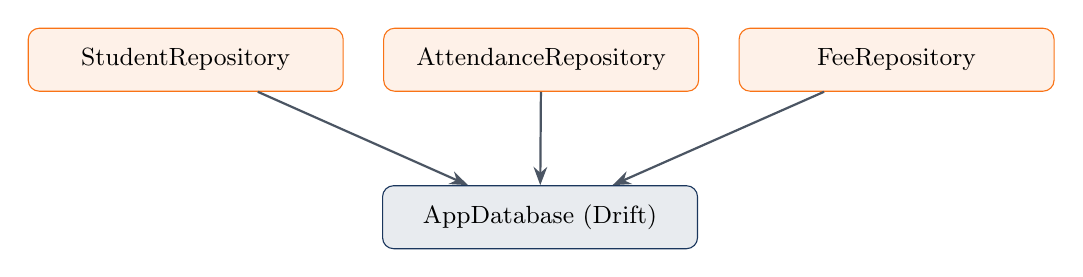
\begin{tikzpicture}[
    node distance=1cm,
    repo/.style={draw=warningorange, rounded corners, minimum width=4cm, 
                 minimum height=0.8cm, fill=warningorange!10, font=\small},
    db/.style={draw=primaryblue, rounded corners, minimum width=4cm, 
               minimum height=0.8cm, fill=primaryblue!10, font=\small},
    arrow/.style={-{Stealth}, thick, darkgray}
]
    \node[repo] (srepo) at (0,2) {StudentRepository};
    \node[repo, right=0.5cm of srepo] (arepo) {AttendanceRepository};
    \node[repo, right=0.5cm of arepo] (frepo) {FeeRepository};
    
    \node[db] (db) at (4.5,0) {AppDatabase (Drift)};
    
    \draw[arrow] (srepo) -- (db);
    \draw[arrow] (arepo) -- (db);
    \draw[arrow] (frepo) -- (db);
\end{tikzpicture}
\end{center}

\subsection{Repository Responsibilities}

\begin{itemize}[leftmargin=*]
    \item CRUD operations on database tables
    \item Complex queries with joins
    \item Data transformation
    \item Caching strategies
\end{itemize}

% ============================================================================
% CHAPTER 5: DATA FLOW
% ============================================================================
\chapter{Data Flow}

\section{Read Operation Flow}

\begin{center}
\begin{tikzpicture}[
    node distance=0.6cm,
    step/.style={draw=secondaryblue, rounded corners, minimum width=3.5cm, 
                 minimum height=0.8cm, fill=lightgray, align=center, font=\small},
    arrow/.style={-{Stealth}, thick, secondaryblue}
]
    \node[step] (ui) {UI Widget};
    \node[step, below=of ui] (consumer) {ref.watch(provider)};
    \node[step, below=of consumer] (provider) {Provider executes};
    \node[step, below=of provider] (service) {Service method};
    \node[step, below=of service] (repo) {Repository query};
    \node[step, below=of repo] (db) {SQLite Database};
    
    \draw[arrow] (ui) -- (consumer);
    \draw[arrow] (consumer) -- (provider);
    \draw[arrow] (provider) -- (service);
    \draw[arrow] (service) -- (repo);
    \draw[arrow] (repo) -- (db);
    
    % Return flow
    \draw[arrow, dashed, primaryblue] (db.east) -- ++(1,0) |- (ui.east);
    \node[right=1.5cm of service, font=\scriptsize, text=primaryblue] {Data flows back};
\end{tikzpicture}
\end{center}

\section{Write Operation Flow}

\begin{center}
\begin{tikzpicture}[
    node distance=0.6cm,
    step/.style={draw=accentgreen, rounded corners, minimum width=3.5cm, 
                 minimum height=0.8cm, fill=lightgray, align=center, font=\small},
    arrow/.style={-{Stealth}, thick, accentgreen}
]
    \node[step] (action) {User Action};
    \node[step, below=of action] (method) {Provider method call};
    \node[step, below=of method] (service) {Service validation};
    \node[step, below=of service] (repo) {Repository write};
    \node[step, below=of repo] (db) {SQLite commit};
    \node[step, below=of db] (notify) {Provider state updated};
    \node[step, below=of notify] (rebuild) {UI rebuilds};
    
    \draw[arrow] (action) -- (method);
    \draw[arrow] (method) -- (service);
    \draw[arrow] (service) -- (repo);
    \draw[arrow] (repo) -- (db);
    \draw[arrow] (db) -- (notify);
    \draw[arrow] (notify) -- (rebuild);
\end{tikzpicture}
\end{center}

% ============================================================================
% CHAPTER 6: MODULE STRUCTURE
% ============================================================================
\chapter{Module Structure}

\section{Feature Modules}

Each feature follows a consistent structure:

\begin{lstlisting}
feature_name/
|-- screens/           # Feature screens
|-- widgets/           # Feature-specific widgets
|-- providers/         # Feature providers (optional)
|-- models/            # Feature models (if not shared)
\end{lstlisting}

\section{Module Dependency Graph}

\begin{center}
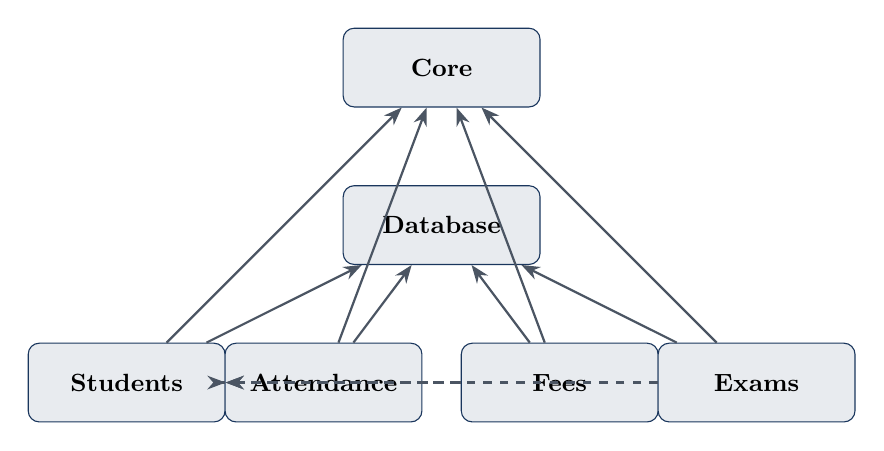
\begin{tikzpicture}[
    module/.style={draw=primaryblue, rounded corners, minimum width=2.5cm, 
                   minimum height=1cm, fill=primaryblue!10, align=center, 
                   font=\small\bfseries},
    arrow/.style={-{Stealth}, thick, darkgray}
]
    % Core modules
    \node[module] (core) at (0,4) {Core};
    \node[module] (db) at (0,2) {Database};
    
    % Feature modules
    \node[module] (students) at (-4,0) {Students};
    \node[module] (attendance) at (-1.5,0) {Attendance};
    \node[module] (fees) at (1.5,0) {Fees};
    \node[module] (exams) at (4,0) {Exams};
    
    % Dependencies
    \draw[arrow] (students) -- (core);
    \draw[arrow] (attendance) -- (core);
    \draw[arrow] (fees) -- (core);
    \draw[arrow] (exams) -- (core);
    
    \draw[arrow] (students) -- (db);
    \draw[arrow] (attendance) -- (db);
    \draw[arrow] (fees) -- (db);
    \draw[arrow] (exams) -- (db);
    
    % Cross-module dependencies
    \draw[arrow, dashed] (attendance) -- (students);
    \draw[arrow, dashed] (fees) -- (students);
    \draw[arrow, dashed] (exams) -- (students);
\end{tikzpicture}
\end{center}

% ============================================================================
% CHAPTER 7: DESIGN PATTERNS
% ============================================================================
\chapter{Design Patterns}

\section{Patterns Used}

\begin{longtable}{@{}p{4cm}p{9cm}@{}}
\toprule
\textbf{Pattern} & \textbf{Application} \\
\midrule
\endhead
Repository & Abstracting data access from business logic \\
Service Layer & Encapsulating business logic \\
Provider/Observer & Reactive state management with Riverpod \\
Factory & Creating complex objects (PDF reports) \\
Singleton & Database instance \\
Dependency Injection & Via Riverpod providers \\
\bottomrule
\end{longtable}

\section{Error Handling}

\begin{lstlisting}[language=Dart]
// Service layer handles all errors
Future<Result<Student>> createStudent(StudentData data) async {
  try {
    final student = await _repository.insert(data);
    await _activityLog.log(action: 'create', entity: student);
    return Result.success(student);
  } catch (e) {
    return Result.failure(AppError.fromException(e));
  }
}
\end{lstlisting}

\end{document}
